%% Common asset library for recurrent neural networks
%%
%% Modular images and common setup for tikz pictures
%%
\usepackage{xargs}
\usepackage{ifthen}
\usepackage{bm}

%% Tikz libraries
\usetikzlibrary{automata,arrows,shapes,matrix,trees,calc,fit,backgrounds,math}

%% Simple network nodes
\tikzset{
  ionode/.style n args={3}{
    circle, thick,
    minimum size=#1,
    inner sep=0pt,
    outer sep=0pt,
    draw=#2!80,
    fill=#2!20,
    label=center:#3,
  }
}
\tikzset{input/.style={ionode={16pt}{blue}{#1}}}
\tikzset{output/.style={ionode={16pt}{red}{#1}}}


%%%%%%%%%%%%%%%%%%%%%%%%%%%%%%%%%%%%%%%%%%%%%%%%%%
%% LSTM command
%%%%%%%%%%%%%%%%%%%%%%%%%%%%%%%%%%%%%%%%%%%%%%%%%%
%% Base on https://duckduckgo.com/?t=ffab&q=lstm+illustration&atb=v1-1&iax=images&ia=images&iai=https%3A%2F%2Fwww.herongyang.com%2FNeural-Network%2FLSTM-Long-Short-Term-Memory-github.png
\tikzset{
  pwiselabel/.style={
    white,
    font=\sffamily\bfseries\tiny
  },
  pwise/.style={
    rectangle,
    inner sep=2.5pt,
    rounded corners=1pt,
    fill=black,
    label={[pwiselabel]center:#1}
  }
}

\tikzset{
  sigtan/.style n args={3}{
    circle,
    minimum size=#1,
    inner sep=0pt,
    fill=#2!80,
    label={center:\tikz\draw[white, thick]  (-#3, -#3) .. controls (#3, -#3) and (-#3, #3) .. (#3, #3);}
  },
  signode/.style={sigtan={12pt}{red}{3pt}},
  tanhnode/.style={sigtan={12pt}{blue}{3pt}},
}

\tikzstyle{lstminnernode}=[circle, inner sep=0, minimum size=1]
\newcommand*{\sigmnode}{
  
\begin{tikzpicture}
    \node [lstminnernode, fill=red!80] at (0, 0) {\fsigmoid{0.08}};
  \end{tikzpicture}
}

\newcommand*{\tanhnode}{
  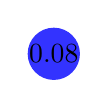
\begin{tikzpicture}
    \node [lstminnernode, fill=blue!80] at (0, 0) {\fsigmoid{0.08}};
  \end{tikzpicture}
}


\newcommand*{\lstm}{
  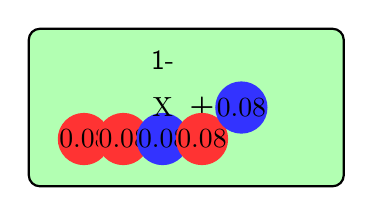
\begin{tikzpicture}[>=latex, thick]
    \draw[rounded corners, fill=green!30] (0,0) rectangle (4, 2);
    \node at (0.7, 0.6) {\sigmnode};
    \node at (1.2, 0.6) {\sigmnode};
    \node at (1.7, 0.6) {\tanhnode};
    \node at (1.7, 1) {\pwise{X}};
    \node at (2.2, 1) {\pwise{$\boldsymbol{+}$}};
    \node at (2.2, 0.6) {\sigmnode};
    % \node at (2.7, 0.6) {\pwise{X}};
    \node at (2.7, 1) {\tanhnode};
    % \node at (0.7, 1.6) {\pwise{X}};
    \node at (1.7, 1.6) {\pwise{\sffamily 1-}};
    
  \end{tikzpicture}  
}
